\documentclass[a4paper, 14pt, oneside]{extbook}
\usepackage[T1]{fontenc}
\usepackage[utf8x]{inputenc}
\usepackage{geometry}
\usepackage{courier}
\usepackage{subfigure}
\usepackage[bookmarks]{hyperref}
\newgeometry{
left=   1.5 in,
bottom= 1.5 in,
right=  1 in,
top=    1 in
}

\usepackage{fancyhdr}

% Grafica
\usepackage{graphicx,pstricks}
\usepackage{graphics}
\graphicspath{{img/}}

% Package usati per il frontespizio
\usepackage{tikz}
\usepackage{pgf-pie}
\usepackage{pgfplots}
\pgfplotsset{width=7cm,compat=1.8}
\usetikzlibrary{patterns}


%Algorithm
\usepackage{algorithm}
\usepackage[noend]{algpseudocode}

\setlength\headheight{44.2pt}
%Page Style
\usepackage{setspace}
%\setstretch{2.5} 
\doublespace

%\cfoot{\thepage}
\lhead[]{}
\rhead[]{\leftmark}

\pagestyle{fancy}{
\lhead{
\includegraphics[scale=0.3]{img/logo/hlogo.png}}
\rhead{\footnotesize{Titolo abbreviato come intestazione}}
}

%Other
\usepackage{comment}
\usepackage{amsmath}

%Testo riempitivo
\usepackage{lipsum}


\begin{document}

%\maketitle
\begin{titlepage}
\thispagestyle{empty}
\raggedright % Allinea a sinistra

\begin{tikzpicture}
\node[anchor=south west] at (4,0) {
\includegraphics[scale=0.75]{img/logo/logo_copertina_1}};
\node[anchor=south west] at (0,1.5) {
\includegraphics{img/logo/logo_copertina_2}};
\node[anchor=south west] at (0,0.5) {\textsf{Scuola Politecnica e delle Scienze di Base}};
\node[anchor=south west] at (0,0) {\textsf{Corso di Laurea Magistrale in Ingegneria Informatica}};
\end{tikzpicture}

\vfill

{\large Tesi di Laurea Magistrale in Big Data Analytics and Business Intelligence}
\\[1cm]
{\textbf{\textit{\LARGE Predictive Mantainance via Anomaly Detection: an approach based on condtional autoencoders}}}
\\[1cm]
{\large Anno Accademico 2019/2020}

\vfill


\begin{table}[h]
Relatore
\\
\textbf{Ch.mo prof. Vincenzo Moscato}
\\
\textbf{Ing. Giancarlo Sperlì}
\\
\textbf{Ing. Antonio Galli}
\\ \\
{\raggedright Candidato}
\\
\textbf{Emanuele Di Fiore}
\\
\textbf{matr. M63000921}
\end{table}

\end{titlepage}
\frontmatter

%\cleardoublepage
%\thispagestyle{empty}
\vspace*{\stretch{1}}
\begin{flushright}
\itshape Una dedica...
\end{flushright}
\vspace{\stretch{2}}
\cleardoublepage

\chapter{Abstract} 

Predictive Maintenance is one of the most important field in the Industry 4.0 era. With the use of Internet of Things (IoT) tools and Information and Communication Technologies (ICT), an huge amount of data related to industrial machinery operating conditions can be collected, enabling and encouraging the use of data-driven approaches for predictive maintenance, especially those based on machine learning and deep learning techniques. With this knowledge, maintenance activities can be planned in optimal way, reducing or even avoiding downtime and saving costs due to unnecessary maintenance procedures.
Anomaly detection is a set of techniques used to understand if conditions in which an industrial machine is working are anomalous or not, only using data collected with a various set of sensors. In last years, many researches started to use deep learning approaches for anomaly detection purposes, encouraged by the great results of these techniques in Computer Vision (CV) and Natural Language Processing (NLP). For example, one of the most used deep learning models is Autoencoder. In fact, even if it is mainly used for dimensionality reduction, autoencoder can be easily adapted to anomaly detection task especially because it allows to resolve its main problem: the absence of sufficient anomalous data to build a classifier. An autoencoder can be trained in unsupervised way, with the absence of anomalous data.\\ Usually, data collected using IoT sensors and then used for anomaly detection range from time-series temperature measurements to equipment vibrations, like bearings, collected by accelerometers. A recent trend is to train autoencoders for anomaly detection using sounds coming from machinery, collected by microphones. In literature, this task in called Anomalous Sound Detection (ASD). Therefore, in this text an unsupervised anomalous sound detection framework based on conditional autoencoders is presented. The main idea is to train the models on sounds belonging to different kinds of the same machine, using their identifiers to condition the latent representation of the autoencoder.\\
To validate the framework, DCASE 2020 Task 2 Challenge dataset is used as a benchmark, because it natively designed for unsupervised anomalous sound detection task. In particular, on the basis of how autoencoder is built, two instances of the proposed framework are implemented: ID Conditioned Convolutional Autoencoder and ID Conditioned LSTM Autoencoder. Results are compared with the baseline model results, provided by the authors of the challenge, and with those found in documentations published by the participants.

{\setstretch{1.5}

\tableofcontents

\cleardoublepage
\addcontentsline{toc}{chapter}{\listfigurename}
\listoffigures

\cleardoublepage
\addcontentsline{toc}{chapter}{\listtablename}
\listoftables

}

\mainmatter

\chapter{Anomaly Detection in Industry 4.0}

% introduzione al capitolo

The first part of this chapter gives some essential definitions about the paradigm of Industry 4.0 and what are its advantages, especially in the context of maintenance. After this brief introduction, an overview of the different approaches to maintenance is presented. Next, the focus is moved to anomaly detection, of which definitions and challenges that must be faced are provided. The chapter ends with an overview of some approaches used in literature to solve anomaly detection tasks, with a spotlight on autoencoder models, providing also the theoretical notions needed to understand the use cases presented in the next chapters.

% titolo della section
\section{Introduction}
The term "Industry 4.0" was used for the first time at the Hannover Fair of Industrial Technologies, in 2011, and refers to the Fourth Industrial Revolution. According to one of the most common definition in literature, Industry 4.0 is a paradigm, a new and innovative way of implementing the industrial processes for the production of a good or a service, thanks to the introduction of the most modern information and communication technologies (ICT), like Cyber Physical Systems (CPS), the Internet of Things (IoT) and Big Data analytics methods.\\ 
The introduction of ICT into core industrial processes allows to take a step forward to the computerization or automation, already introduced with the third industrial revolution, especially in the manufacturing industry: a simple factory becomes smart with integration of different physical and digital systems, from the production sectors to marketing or logistics ones, through devices, called smart sensors. Smart sensors allow the creation of a machine-to-machine interaction without the interventions of human operators \cite{1smartfactory}, enabling also the collection of a large amount of data like measurements of temperature, humidity, vibration speed or sound of an equipment for monitoring automations and process configurations improvements. This large amount of data can also be useful to assess the current health status of machines and to plan maintenance activities, which have the main goal of reducing the unexpected downtime and expensive costs due to failures occurrences. Moreover, this new paradigm helps the improvement of new business models and allows to satisfy the emerging demand of products customization through an intelligent process control and management.

\section{Maintenance approaches}
Maintenance is the combination of all technical, administrative and managerial necessary actions during the life cycle of an item (in our context a machine) intended to restore it to a state in which it can perform better what it is designed for \cite{4maintenanceTransformation}. It is clear that maintenance activities are not only the physical operations that are needed to repair a particular machine, but also all activities for the planning and the scheduling of such operations, together with cost analysis. For these reasons, maintenance plays an important role in ensuring the success of a manufacturing company due to its impact on productivity, quality of products and companies economic balances.\\
In literature, several maintenance approaches can be found \cite{3SystematicLiteratureReviewML}. Three strategies are listed below, also summarized by the Figure \ref{maintenance_strategy_overview}:

\begin{itemize}
\item{\textit{Run-to-Failure (R2F)} or \textit{Corrective maintenance} consists in repairing an equipment when it stops working. This is the simplest strategy, but also the less convenient one because it is necessary to stop the production in order to repair or replace the components that create problems.}
\item{\textit{Preventive Maintenance (PvM)} or \textit{Time-based Maintenance} is more effective than R2F but it increases the operating costs because some times these corrective actions are scheduled when unnecessary.}
\item{\textit{Predictive Maintenance (PdM)} uses some prediction tools to establish when maintenance is necessary. It allows a continuous monitoring of machines status and an early detection of failures, avoiding unnecessary actions.}
\end{itemize}

\begin{figure}[ht]
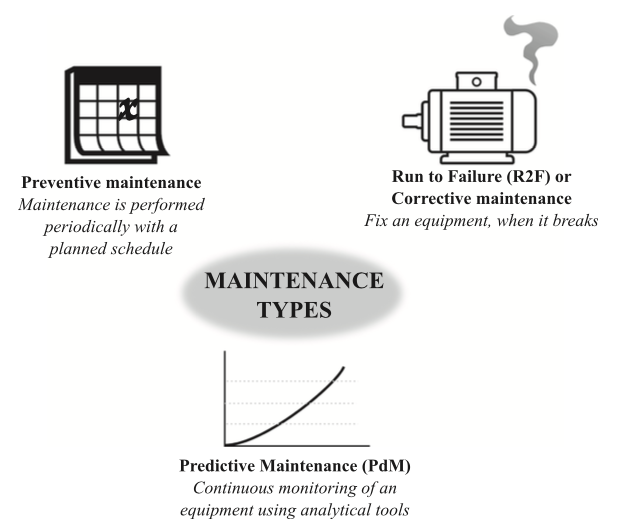
\includegraphics[scale=0.9]{TESI DI FIORE/img/maintenance_strategy_overview.png}
\centering
\caption{Overview of different maintenance strategies \cite{3SystematicLiteratureReviewML}}
\label{maintenance_strategy_overview}
\end{figure}

Therefore, an optimal maintenance strategy should improve the equipment conditions for a better quality of final products, reduces equipment failure rates to minimize downtime in production, maximizes equipment lifetime and minimizes the total costs. According to this, the PdM is the most promising strategy and the one that is under the researcher's spotlight in the last few years. \\ 
Citing the study realized by Thyago P. Carvalho et al. \cite{3SystematicLiteratureReviewML} and Weiting Zhang et al. \cite{2DataDrivenMaintenance}, the PdM methods are mainly divided into three categories: 
\begin{itemize}
\item{\textit{Model-Based Predictive Maintenance} consists in the development of complex mathematical models which replicate the behaviour of an equipment and its degradation process.}
\item{\textit{Knowledge-Based Predictive Maintenance} consists in the application of threshold-based rules, built on some measurements taken from machines, and that generate alerts in case in which some of them cross the thresholds.}
\item{\textit{Data-Based or Data-Driven Predictive Maintenance} makes the use of progresses reached in the fields of advanced analytic and artificial intelligence (AI) techniques to build machine learning (ML) or deep learning (DL) models that have the capability to predict when next failures will occur. }
\end{itemize}

It is good to clarify that behind the word "predictive" several meanings are hidden. In data-driven techniques the main goal is to train ML or DL models on historical data, which contains information about the degradation of a component or about normal or anomalous behaviour of an equipment, and then use them to predict its remaining useful life (RUL) or to detect some anomalies and generate alerts. Obviously this category of PdM is boosted by the paradigm of Industry 4.0 thanks to the large amount of historical or real-time time-series data collected by sensors in smart factories, allowing ever better performances.\\
The main drawback of using Industry 4.0 paradigm, especially to enable predictive maintenance, is the cost of digitalization, but fortunately in last years European Governments has started to support this transition defining new and accurate plans of investment in research and development. For example, the Italian government, with the "New Transition Plan 4.0", published in 2020 and valid for the next three years, is going to invest around 24 billion euros to promote the digital transition and to support investments by private companies \cite{12MiseNuovoPianoTransizione}.\\ 
In conclusion, regarding tangible results of the transition, is worth analyzing the Figure \ref{predictive_maintenance_reduction_costs}, taken from the study made by Porsche Consulting \cite{11PorscheStudy}, which results show a significant reduction in maintenance costs through implementation of predictive systems.

\begin{figure}[ht]
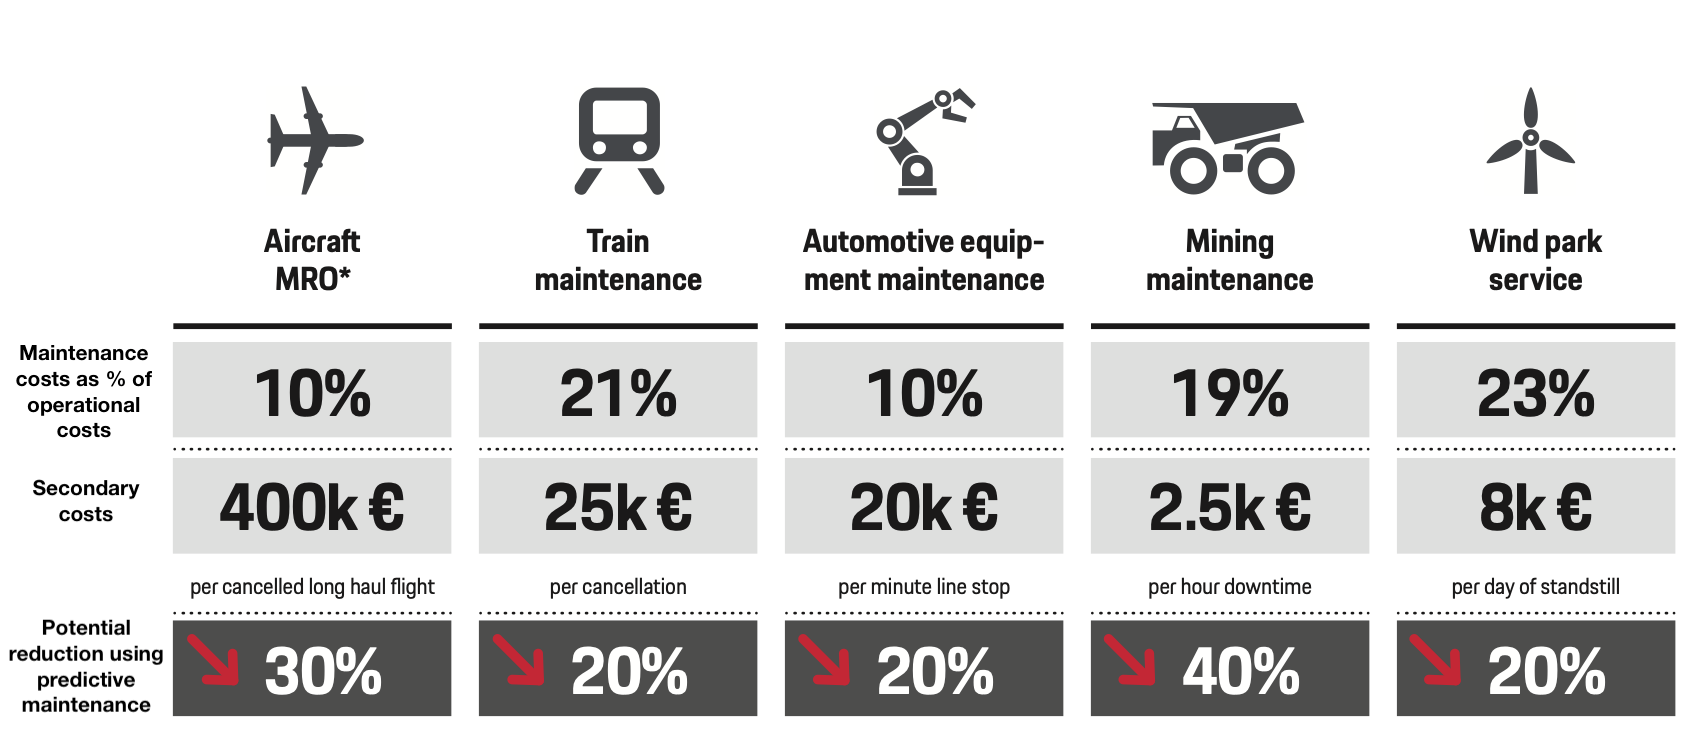
\includegraphics[scale=0.4]{TESI DI FIORE/img/UsingPredictiveMaintenanceCostReduction.png}
\centering
\caption{Potential overview for maintenance cost reduction across five industries \cite{11PorscheStudy}}
\label{predictive_maintenance_reduction_costs}
\end{figure}


\section{Anomaly Detection in PdM}
Anomaly detection (or outlier detection) is a set of techniques for the identification of anomaly patterns in data that deviates from normal behaviour. For example, a machine, like a pump or a steam turbine, after a period of normal behaviour starts deteriorating due to regular use, generating some \textit{anomalies} and entering in a status that can be identified as anomalous. This state should not be considered as a total failure state (in such case the machine should be turned off) but as a warning state, indicating that some maintenance procedures are needed \cite{5AnomalyDetectionSurvey}. Anomaly detection is so used to minimize the cost of failures, discovering anomalous behavior of mechanical devices in the production line in order to predict potential problems as early as possible. In this way, the production plans can be adjusted accordingly to avoid failures, and the failures already happened can be contained in their early stage to avoid cascading effects.\\
As for the PdM in general, in last years, in the context of anomaly detection, different ML and DL techniques have been developed. Most of them are based on time-series, which represents historical or real-time measurements of different parameters recorded in sequence from machines by smart sensors. In this type of data, three different kinds of anomaly can be identified \cite{6AnomalyIoTTimeSeries}: 
\begin{itemize}
\item{\textit{Point anomaly}: the time-series returns in normal state in very short time period, so the anomaly is represented by only few observations;}
\item{\textit{Contextual anomalies}: observation or sequences that deviates from expected patterns, but if taken in isolation they not exceed the range of expected values for that signal;}
\item{\textit{Collective or Pattern Anomalies}: observations that are labeled as anomalous only if taken together.}
\end{itemize}
In the Figure \ref{anomalies} can be found a graphical view of the just mentioned anomaly types. 
\begin{figure}[ht]
\centering
\begin{subfigure}
    \centering
    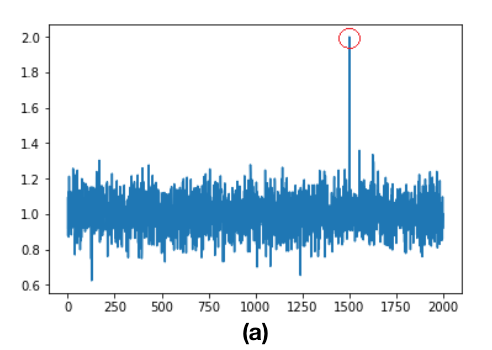
\includegraphics[scale=0.51]{TESI DI FIORE/img/anomaly_a.png}
\end{subfigure}
\begin{subfigure}
    \centering
    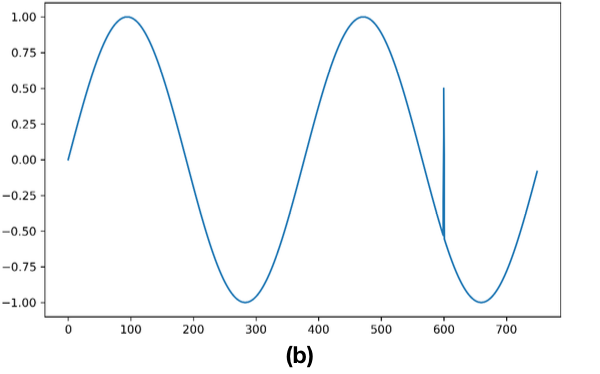
\includegraphics[scale=0.45]{TESI DI FIORE/img/anomaly_b.png}
\end{subfigure}
\begin{subfigure}
    \centering
    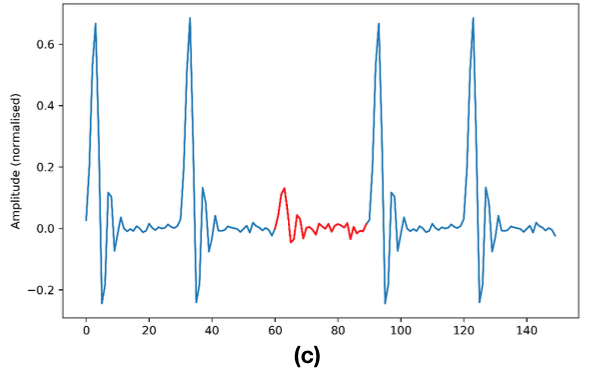
\includegraphics[scale=0.45]{TESI DI FIORE/img/anomaly_c.png}
\end{subfigure}
\caption{Point anomaly (a), contextual anomaly (b) and collective anomaly (c) \cite{6AnomalyIoTTimeSeries}.}
\label{anomalies}
\end{figure}

\section{Challenges of Anomaly Detection}
Being a field of predictive maintenance, also in anomaly detection there are some important elements that must be taken into consideration, because they influence the performances of trained models.
\subsection{Contextual information}
The presence of a variety of sensors, distributed around the environment of the monitored system, gives the opportunity to include contextual information into the collected data, allowing the improvement of the anomaly detection process performances. In particular, two types of contexts must be handled: spatial context and external context. When multiple sensors are deployed to monitor a system that moves in different environment conditions, such as a train, the contextual information can effect a lot the performances of an anomaly detector. For example some behaviours that are normal when a train is running on a flat ground can be anomalous when it is climbing an incline. This problem could be resolved using an accelerometer that measures the angle with the ground and incorporate its observations during the training. Moreover, external context can be likewise effective when monitoring the internal temperature of an equipment, because in this case the knowledge of external temperature can effect the results of the detection in better. Obviously, taking in consideration the context, some drawbacks are present, for example the necessity to build a more complex and expensive monitoring system and a more difficulty in model training.
\subsection{Data dimensionality and noise}
Other important elements that must be taken in consideration into the development of an anomaly detector are the data dimensionality and measurements noise. Regarding data dimensionality, there are two different cases: univariate or multivariate data. Univariate data consists of observations recorded by a single sensor, while multivariate data consists of a sequence of observations recorded by multiple sensors. In the first case, machine learning models must be trained to discover the historical relationships that could be hidden in the sequence of values recorded by one sensor. In the second case, observations recorded by more than one sensor are linked together by the timestamp. This can be regarded as an advantage in some situations in which patterns are hidden between the relationships among the various physical measures monitored by sensors. Regarding the noise, in an IoT environment where a large number of low cost, resource constrained sensors are deployed, the data quality is often affected by significant disturbs, inconsistencies and missing or duplicated data. Where the sensors are powered by battery, these challenges are often amplified as the available charge decreases. These problems can be resolved aggregating data from multiple similar sensors into a single observation to reduce the environmental noise.
\subsection{Stationarity}
Stationarity is also another important element that needs to be treated: a stationary time-series is one where the mean, variance and autocorrelation does not vary with time. Unfortunately, in real world non-stationary time series are very frequent and this make more complex the training of AI models because statistical data stream distribution may vary over time and so what is normal over a period of time could be anomalous in another (concept of seasonality).
\subsection{Lack of anomalous data}
One last challenge, maybe the most important that must be faced in anomaly detection, is the prediction of the "unknown". The word "unknown" refers to undesirable (or anomalous) events of which available data are not enough. The consequence is that ML and DL models can not be trained using a classification approach, because only normal state monitored data of an equipment are available to build an anomaly detector \cite{7AnomalyDetectionUnsupervised}. In fact, for example, while it is possible to build a toy industrial machine in order to collect data of its normal and anomalous working states, on the other hand, in some situations, it is unthinkable, dangerous and expensive try to generate anomalous behaviors of a machinery used in real world, like an aircraft engine, a train engine or an industrial press, with the only goal of collecting data. Moreover, even if anomalous data are available, they not surely represent all the anomalous situations in which the machine under investigation could be, because the space of the anomalies is very irregular and it is practically impossible to have a complete vision of them in order to trains models with a classification approach.

\section{Unsupervised Anomaly Detection}
Because is quite simple to collect large dataset associated to a particular machine's working state, in such situations, ML and DL models must be trained in a unsupervised way, where the word unsupervised means that the models try to detect an events that have no examples in the data history used for training \cite{8AnomalyDetectionUnsupervised2}. At this point, a question that arises is: how a trained model could detect never seen anomalous measurements and generate alerts? A possible approach is showed in Figure \ref{scoring_system_approach}. The figure shows that models could be trained to reconstruct the received input, that refers to a normal working state, and if the output is enough different from the input an alert will be triggered.

\begin{figure}[ht]
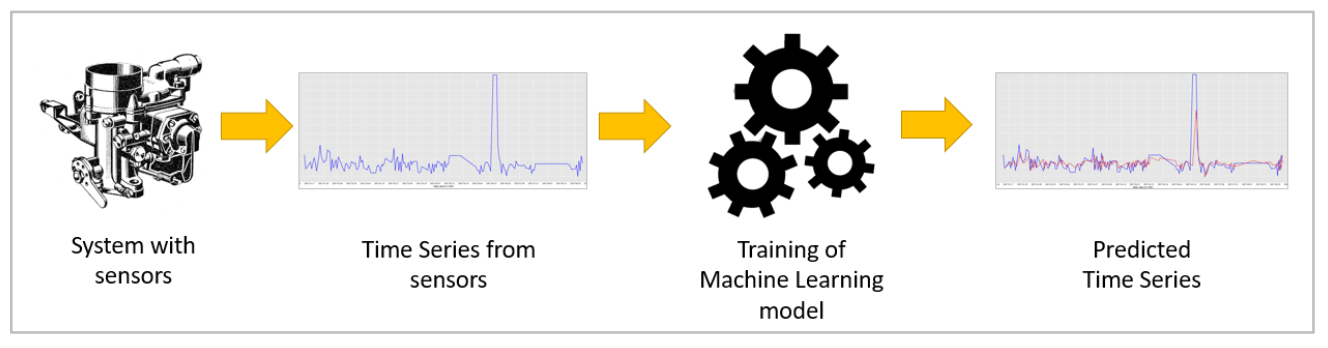
\includegraphics[scale=0.65]{TESI DI FIORE/img/UnsupervisedLearningAnomalyDetection.png}
\centering
\caption{Anomaly detection high level workflow \cite{7AnomalyDetectionUnsupervised}}
\label{scoring_system_approach}
\end{figure}

Anomalies in sensor data can be defined as previously unseen patterns and the algorithm for anomaly detection should be able to detect known anomalies as well as generalize to new and unknown ones. In general, a common approach to achieve this detection is a sliding-window (Figure \ref{anomaly_detection_with_sliding_window}). Since medels are trained on normal data which is a fixed-length sequence of preceding steps, it can achieve anomaly detection by comparing the predicted value at each timestep with the actual sequence, allowing also to perform a real-time detection and eventually alerts generation \cite{9UnsupervisedOnlineAnomalyDetectionMultivariate} and, moreover, using the temporal relationships present in sequences.
\begin{figure}[ht]
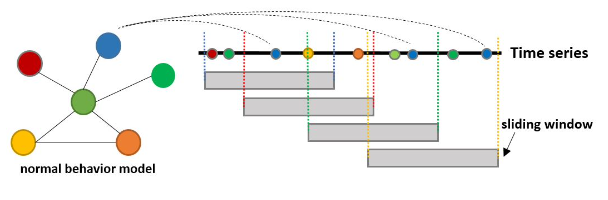
\includegraphics[scale=0.8]{TESI DI FIORE/img/OnlineAnomalyDetection.png}
\centering
\caption{Online detection procedure with sliding window \cite{9UnsupervisedOnlineAnomalyDetectionMultivariate}}
\label{anomaly_detection_with_sliding_window}
\end{figure}
Several approaches have been developed for unsupervised anomaly detection. R. Silipo et al \cite{8AnomalyDetectionUnsupervised2} describes two techniques: the first, named Control Chart, and the second based on Auto-Regressive (AR) models. In the first case, the boundaries for an anomaly-free functioning equipment are defined. This boundaries are usually centered on the average signal values recorded by sensors and bounded by twice the standard deviation in both directions. If the signal is wandering off this anomaly free area, an alarm should occur. The second approach is conceptually similar to the Control Chart and uses this anomaly-free time window to train an AR model. The boundaries for anomaly-free functioning are defined here on the prediction errors on the training set. To clarify, the model receives in input a time-series made by sensor observations and the next time-step value is then predicted by the model. Successively, according a threshold established using the training set, if the predicted value is enough different from the actual value, an alarm is fired off requiring further checkups. This second technique is also cited in the survey \cite{6AnomalyIoTTimeSeries}.\\
Another important and suitable machine learning method for this task is \textbf{autoencoder} and for this reason it will be at the center of this discussion. 
An autoencoder (Figure \ref{autoencoder_image}) is a neural network mainly designed to encode the input into a compressed and meaningful representation and then decode it back, such that the reconstructed input is as much as similar to the original one \cite{10Autoencoders}.\\
\begin{figure}[ht]
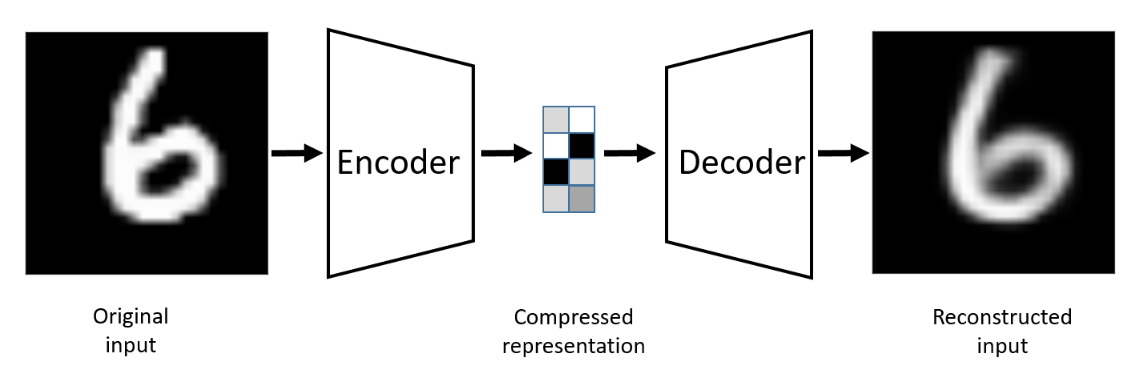
\includegraphics[scale=0.65]{TESI DI FIORE/img/Autoencoder.png}
\centering
\caption{An autoencoder example \cite{10Autoencoders}.}
\label{autoencoder_image}
\end{figure}
Autoencoder is so an unsupervised technique because any label or class is needed for training phase, so it results a perfect approach for anomaly detection. In details, the encoder part is made of a series of layers with a decreasing number of nodes and ultimately reduces data into a latent vector, which represents a reduced (encoded) version of the input and which contains only valuable or essential information of it. The decoder, as the encoder, is made of different layers with an increasing number of nodes. It is trained to receive in input the latent vector and to generate an output as much as possible similar to the input. The process is described in mathematical way as follow:
\[argmin_{D,E} || X - D(E(X))||\]
Where X is the input data, E is an encoder network, and D is a decoder network. Using this formula is evident that the performances of an autoencoder are evaluated using the reconstruction error: the difference between the input and the output in terms of mean absolute error (MAE) or mean squared error (MSE).\\
Summarizing, in the context of anomaly detection in predictive maintenance, the autoencoder can be trained to reconstruct the normal observations collected from a working machine in normal working state. Next, in detection phase, its reconstruction error can be used as an anomaly score: if it is under a threshold the observation in input can be classified as normal, otherwise as anomalous. As mentioned before for AR models, the threshold is found using the reconstruction error of training set samples or using different techniques.\\
The next chapter presents different autoencoder approaches in anomaly detection, with a particular focus on anomalous sound detection tasks.


\chapter{Related Works}

This chapter presents, in the first section, an overview of the different datasets available online for anomaly detection tasks. Next, different autoencoder-based architectures found in literature are presented.

\section{Available datasets}
One of the main reasons for the success of ML or DL algorithms in last years is the availability of more and more public standard datasets, regarded as common benchmarks and that consequently allow a fair comparison between different proposals in literature. In PdM and in anomaly detection tasks, this is not totally true because often machinery data are confidential and sometimes studies are conducted by companies' internal divisions and the consequence is that observations are not made available publicly. In response to this need, in the last years some datasets have been built and then made available online (Table \ref{datasets-table}).\\

% Please add the following required packages to your document preamble:
% \usepackage{booktabs}
\begin{table}[ht]
\small
\centering
\begin{tabularx}{\textwidth}{cl}
\hline
Dataset Name & Summary \\ \hline
CWRU & \begin{tabular}[c]{@{}l@{}}Ball bearing test data for normal and faulty bearings. \\ Motor bearings were seeded with faults using electro-discharge\\ machining (EDM) and vibration data was collected using \\ accelerometers, which were attached to the housing \\ with magnetic bases.\end{tabular} \\ \hline
MFPT & \begin{tabular}[c]{@{}l@{}}Provides time-series data from nominal, outer race fault at \\ various loads, inner race fault at various loads and three\\ real-world faults of bearings\end{tabular} \\ \hline
NAB & \begin{tabular}[c]{@{}l@{}}Contains cross-domain data collections, like \\ the average CPU usage in AWS cluster or the internal \\ temperature data of an industrial machine.\end{tabular} \\ \hline
Yahoo S5 & \begin{tabular}[c]{@{}l@{}}Consists of four data classes, each of which contains either a\\  set of synthetic or real web traffic metrics tagged with anomalies\end{tabular} \\ \hline
DCASE2020 & \begin{tabular}[c]{@{}l@{}}The dataset consists in sounds collected \\ from different industrial machines. It is composed by MIMII \\ Dataset and ToyADMOS.\end{tabular} \\ \hline
\end{tabularx}
\caption{Anomaly detection online available datasets.}
\label{datasets-table}
\end{table}

To clarify, these datasets contain some anomalous observations generated manually by operators, but, as mentioned in the first chapter, they not represents all the possible anomalous states and they are only used to build test set and consequently evaluate the performance of the models, trained in unsupervised way with the use of only normal states data. 

\section{Anomaly detection with autoencoders}
In this section, some autoencoder-based architectures found in literature are presented.
Antonio L. Alfeo et al. \cite{12UsingAEinManufacturing} show an autoencoder-based approach with different case studies addressing industrial laundry assets’power consumption and bearing vibrations. In the first case, the time-series data are realistically created using the official information of assets’ manufacturers (e.g. nominal energy consumption) and the details provided by researchers' industrial partner. In the second case, time-series are extracted from MFPT dataset presented in Table \ref{datasets-table}. After the creation of these ad-hoc datasets, the proposed approach employs an autoencoder to score the anomaly degree of each input instance (presented as rescaled time-series features), after it has been trained with regular occurrences. The reconstruction errors, calculated downstream of the decoder, are further processed by the discriminator, which rescales them between 0 and 1 by using a sigmoidal function (Figure \ref{autoencoder_plus_discriminator}).
\begin{figure}[ht]
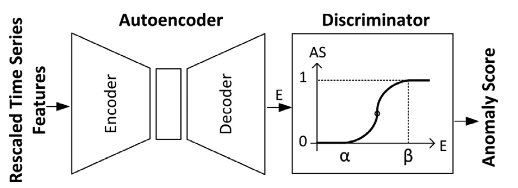
\includegraphics[scale=0.7]{TESI DI FIORE/img/Autoencoderplusdiscriminator.png}
\centering
\caption{Anomaly detector architecture proposed by \cite{12UsingAEinManufacturing}.}
\label{autoencoder_plus_discriminator}
\end{figure}
For both the dataset, the inputs of the architecture are samples characterized by statistical features extracted from time-series available in the dataset which capture their trends of them over time (like 90th, 75th, 50th and 25th percentile of the time series or the mean absolute deviation).\\
Ruei-Jie Hsieh et al \cite{9UnsupervisedOnlineAnomalyDetectionMultivariate} developed an unsupervised deep RNN (Recurrent Neural Network) detection model based on the LSTM (Long Short Term Memory) autoencoder. The recurrent layers of the autoencoder allow to capture temporal dependencies in multivariate sensor data provided by a manufacturing company. The mentioned company has a production line in which there are three chambers (A,B,C) disposed in series and the product moves from a chamber to another. Each chamber has 4 sensors (W,X,Y,Z) for the detection of the products passage. When sensors outputs signal 1, it indicates the product is already in a chamber, otherwise it outputs 0. Obviously, the anomalies in data are not detectable in the single values generate by sensors, but only in the time sequence of them. This is the reason of using LSTM cells to build encoder and decoder layers. The detection of an anomalous behaviour in a chamber prevents that the products pass in the whole production line (early detection). Autoencoder models are trained to reconstruct input sequences, timestamp by timestamp, using a sliding-window method (sequence-to-sequence autoencoder). The input vector in each timestamp is composed by the outputs of the four sensors in a chamber. Using a threshold $\epsilon$, defined using the reconstruction error of training data, each timestamp of each sequence is labeled as normal or anomalous on the basis of its reconstruction error. In conclusion, as each timestamp is labeled as many time as the sliding window length, a majority voting mechanism is applied to make the final decisions and eventually an alert is generated (Figure \ref{seq2seq-architecture}).
\begin{figure}[ht]
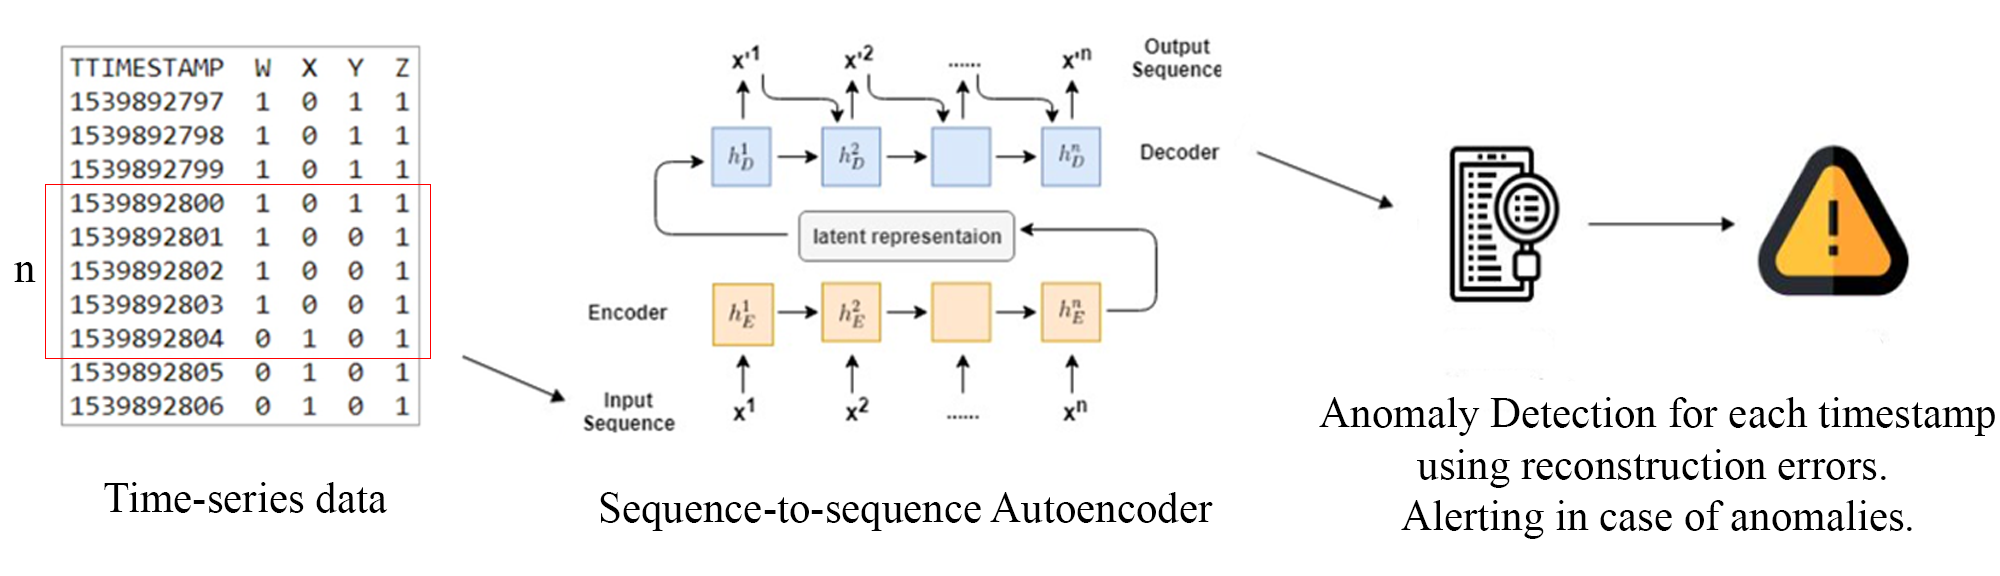
\includegraphics[scale=0.9]{TESI DI FIORE/img/sequence-to-sequecen-ae-anomalydetection.png}
\centering
\caption{Architecture pipeline proposed by \cite{9UnsupervisedOnlineAnomalyDetectionMultivariate}.}
\label{seq2seq-architecture}
\end{figure}\\
Another strategy to resolve the anomaly detection task is to combine deep learning and ensemble learning. Shao Haidong et al. \cite{14NovelMethodEnsembleDeepAutoencoder} propose a novel method called ensemble deep autoencoders (EDAEs) for the intelligent fault diagnosis of bearings, using CWRU dataset. The ensemble of multiple deep autoencoders is a good choice to overcome the low generalization ability of individual deep autoencoders. Diversification is obtained by designing deep autoencoders with different kind of activation functions, because neural networks differing in activation functions usually show different characteristics and complementary learning behaviours. As combination strategy, the authors define a new one. For each deep autoencoder the classification accuracy is calculated and then compared to a pre-defined threshold. Only autoencoders with accuracy greater than the threshold are kept. Using accuracies, different weights are calculated and then assigned to each model and at the end, the achitecture reports the combined diagnosis result of each sample based on the weight scores. In order to maintain the stability of the combined diagnosis results, repeated trials are carried out. The results (in terms of precision, recall and F-Measure), shown in the paper, demonstrate the validity of this architecture.\\
The existing anomaly detection systems used in the industrial domain depend on the properties of sensors. Among those systems, most common are visual anomaly detection systems, which have some drawbacks such as illumination, occlusion by objects, being out of the field of view, and so forth, which strongly affect the performance of the system, also in terms of computation power needed to achieve real time performance. The Anomalous Sound Detection (ASD) systems, however, are not affected by the problems just described, and thus offer an advantage using acoustic data features, especially in terms of computation power needed for real time detection and of simplicity in collecting data. A drawback of using acoustic data is that they must be transformed to be compatible with the training processes of autoencoder models. In fact, compared to images, audio clips need some pre-processing steps in order to convert them in different formats compatible with neural network training process, like signals composed by air pressure values or spectrograms, often in the Mel scale\footnote{Mel spectrograms derive from a particular cepstral representation of the audio signal. The difference between the cepstral and the mel-frequency cepstral representation is that, in the MFC one, the frequency bands are equally spaced on the Mel scale, which approximates the human auditory system’s response more closely than the linearly-spaced frequency bands used in the normal cepstral transformation.}.\\
In this context, the authors of \cite{13RealTimeDetectionUsingSequentialAutoencoder} compare the performances of convolutional LSTM autoencoder (Conv-LSTMAE)  and sequential convolutional autoencoder (CAE) using sounds retrieved from Youtube videos recorded during industrial manufacturing processes. Because it is hard to capture abnormal patterns due to their rarity in real life and because the creation of anomaly events and recording respective sounds is expensive, the authors generate artificially anomalous samples for testing adding anomaly events like explosion, fire or glass breaking to downloaded clips. Although the proposed two autoencoders are different in terms of layers, the pipeline of the system is fixed: there are sequences of five 128x128 spectrograms (extracted from audio dataset) that are the inputs of sequence-to-sequence encoding and decoding networks, which generate output sequences that must be as much as similar to the input ones. Also this time, the decision about the generation of an alert due to the possible presence of anomalies, is made on the comparison between the reconstruction error of each spectrogram to a pre-defined threshold.

\section{Anomalous sound detection with DCASE dataset}
Detection and Classification of Acoustic Scenes and Events, is a community that organizes challenges every year and usually their task 2 regards machineries sound data. The dataset presented in the Table \ref{datasets-table} is provided by DCASE 2020 Challenge, which title is "\textit{unsupervised detection of anomalous sounds for machine condition monitoring}". Because of only normal working machines sound samples are provided as training data (in form of clips, lasting 10 or 11 seconds), the task must be resolved in unsupervised way, and again autoencoder is one of the best unsupervised approach to do this. In details, the dataset that can be downloaded is composed by ToyADMOS Dataset and MIMII Dataset \cite{DCASE} and refers to different sounds recorded with microphones disposed around different machine types: a Toy-car, a Toy-Conveyor, a valve, a pump, a fan and a slide rail. To make the challenge more interesting, for each machine type different kinds of machines are considered, identified by a numeric ID (for example different kinds of pump). A baseline system implementation for comparison purpose was made available by the authors of the challenge. It consists of a dense autoencoder with three layers, in both the encoder and decoder components, with 128 units, and a latent space with 8 units, all with the ReLU activation function. Following, a summary of most interesting approaches to improve the baseline system is shown, while, in the next chapters, the dataset is explored more in details to support a better explaination of the experimental part of this work.\\
% LITERATURE
Pilastri et al. \cite{15DeepDenseConvAE} propose two deep learning models, based on a dense and convolutional architectures fed with Mel spectrograms. For the dense one, the encoder and decoder networsks consist of four fully-connected layers, followed by Batch Normalization and ReLU as the activation function. For the convolutional one, the encoder and decoder networks are comprised of convolutional layers with Batch Normalization and the ReLU activation function after each convolution. In both architectures the goal is to minimize the reconstruction error between inputs and outputs. Regarding features extraction, for the dense autoencoder, audio samples are buffered in fixed-length 1 second intervals with a 50\% overlap and, after the extraction of Mel spectrograms 128x640 dimensional input matrix are obtained. In the convolutional autoencoder system, the mel spectrograms obtained from samples are segmented to form 128x32 frames, ready for training. As for previous described architectures, the classification of audio clips, is made comparing the reconstruction error (in terms of mse) and a pre-defined threshold. Results show that for two machine types (slider and valve), the best results were achieved by the convolutional autoencoder, while the dense autoencoder provided the best results for the others.\\
Again, also in anomalous sound detection task, some LSTM-based autoencoders architecture can be found in literature. For example, in the technical report provided by Jalali et al. \cite{16LSTMDeepAutoencodersForASDtask}, the architecture encodes the information using LSTM layers with \textit{n} units and then their outputs are passed into a bottleneck layer, which is also a LSTM layer with smaller size together with a repeat vector layer. A repeat vector layer repeats its input vector multiple times (the number of time steps chosen for the sequences). Next, a stack of sequential LSTM layers reconstruct the original input.\\
Another interesting approach is the one proposed by Tomoki Hayashi et al. \cite{17ConformerBasedIDAWAREAutoencoder}. Their paper presents a Transformer-based and Conformer-based autoencoder for ASD, performing sequence-by-sequence processing. As opposed to the standard autoencoder, this kind of architectures can extract sequence-level information from whole audio inputs, using a methodology called self-attention mechanism, with whom Trasformer and Conformer neural networks are built. In fact, a critical disadvantage classic sequence-to-sequence autoencoder is the inability of the system to retain longer sequences. The attention mechanism was created to resolve this problem of long dependencies, as it is an interface connecting the encoder and decoder providing to the decoder the information from every encoder hidden state. With this framework, the model is able to selectively focus on valuable parts of the input sequence and hence, learn the association between them.\\
As can be noted, all the approaches proposed above differ from the way autoencoders are built. In fact, the main idea is always to train autoencoders to reconstruct as well as possible the normal audio samples provided in input and then to detect anomalies when there is some input that are badly reconstructed by the architecture. In literature, however, there are also some proposals that are regardless of how the autoencoders are build. For example, the authors of \cite{18IDConditionedAutoEncoder}\cite{19DescriptionDiscussionDCASE2020} and also the same researchers of the last presented approach, introduce the concepts of ID conditioning and ID regression. The main idea of both is to use the information related to the particular device identifier from which the input sound clips is retrieved to influence the autoencoder behaviour. In case of ID embedding, the machine ID (which identifies the brand of the particular machine type) is concatenated or added to the latent variables extracted by the encoder. This makes possible to inform the decoder of the machine ID information explicitly, allowing the training of only one model for the all the available machine brands. In the case of the ID regression, the idea is to concatenate the machine ID to the input features, and the autoencoder then reconstructs not only the input acoustic features but also the machine ID. The reason of this is that the autoencoder tends to confuse the machine ID when the audio clip includes an anomalous sound even if the correct machine ID is provided as the inputs. Therefore, the model can detect whether the audio clip includes an anomalous sound from the estimated machine ID.
\chapter{Proposed Framework}
As already shown, one of the main task of predictive maintenance is anomaly detection, described as a set of techniques for the identification of some anomalous warning states in which an under observation machine could be, allowing a better maintenance activities planning. In this part, the task performed is firstly formalized and then the proposed architecture is illustrated. At the end of the chapter a list of technologies used during implementation is presented.
\section{Problem definition}
In this section the performed anomalous sound detection task is formalized. The proposed framework is built to classify as normal or anomalous audio clips placed in input. The training set is composed of $K$ audio clips $\{x_1, x_2, ...,x_K\}$ in \textit{.wav} format, recorded from different versions of a machine type $M$, with a duration of $T$ seconds (for example $K$ clips from four different pumps). An ID string is used to identify the different versions of $M$. Moreover, since only few audio clips are recorded when anomalies are present, they are incorporated into a different set, used for testing purpose. For the reasons explained in previous chapters, this task cannot be solved using classification, even though it seems to be a two-class classification problem. To clarify, only one model is trained to perform anomaly detection on different versions of M, using, in training phase, normal audio clips recorded from all of them. In this way the complexity of the predictive maintenance system is reduced, because one single model can be used for different machines, avoiding repeating the training operations, in any case expensive, for each machine.\\
Before describing the proposed model in detail, let’s have a look to the implemented framework from an high level view (Figure \ref{high-level-architecture}). As it can be seen, the input consists in an audio clips recorded by microphones disposed around monitored machines, while the output is a label, \textit{normal} or \textit{anomaly}.
\begin{figure}[ht]
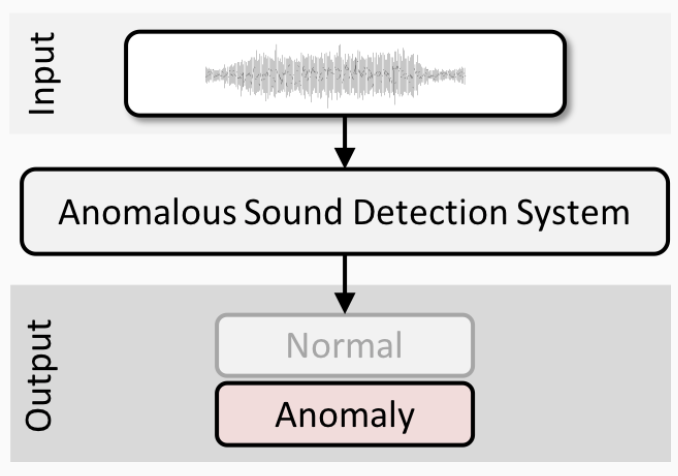
\includegraphics[scale=0.6]{TESI DI FIORE/img/high-level-architecture.png}
\centering
\caption{High level architecture \cite{DCASE}}
\label{high-level-architecture}
\end{figure}

\section{Model architecture}
The proposed ASD system operations, shown in Figures \ref{offline-asd-system} and \ref{online-asd-system}, consist of two main phases: an offline phase, responsible of autoencoder models training, and an online operation phase, to conduct a real time detection.\\
In the next two subsections there are detailed descriptions of both phases, with a focus on each block present in the pipelines.
\subsection{Offline Training Phase}
\begin{figure}[ht]
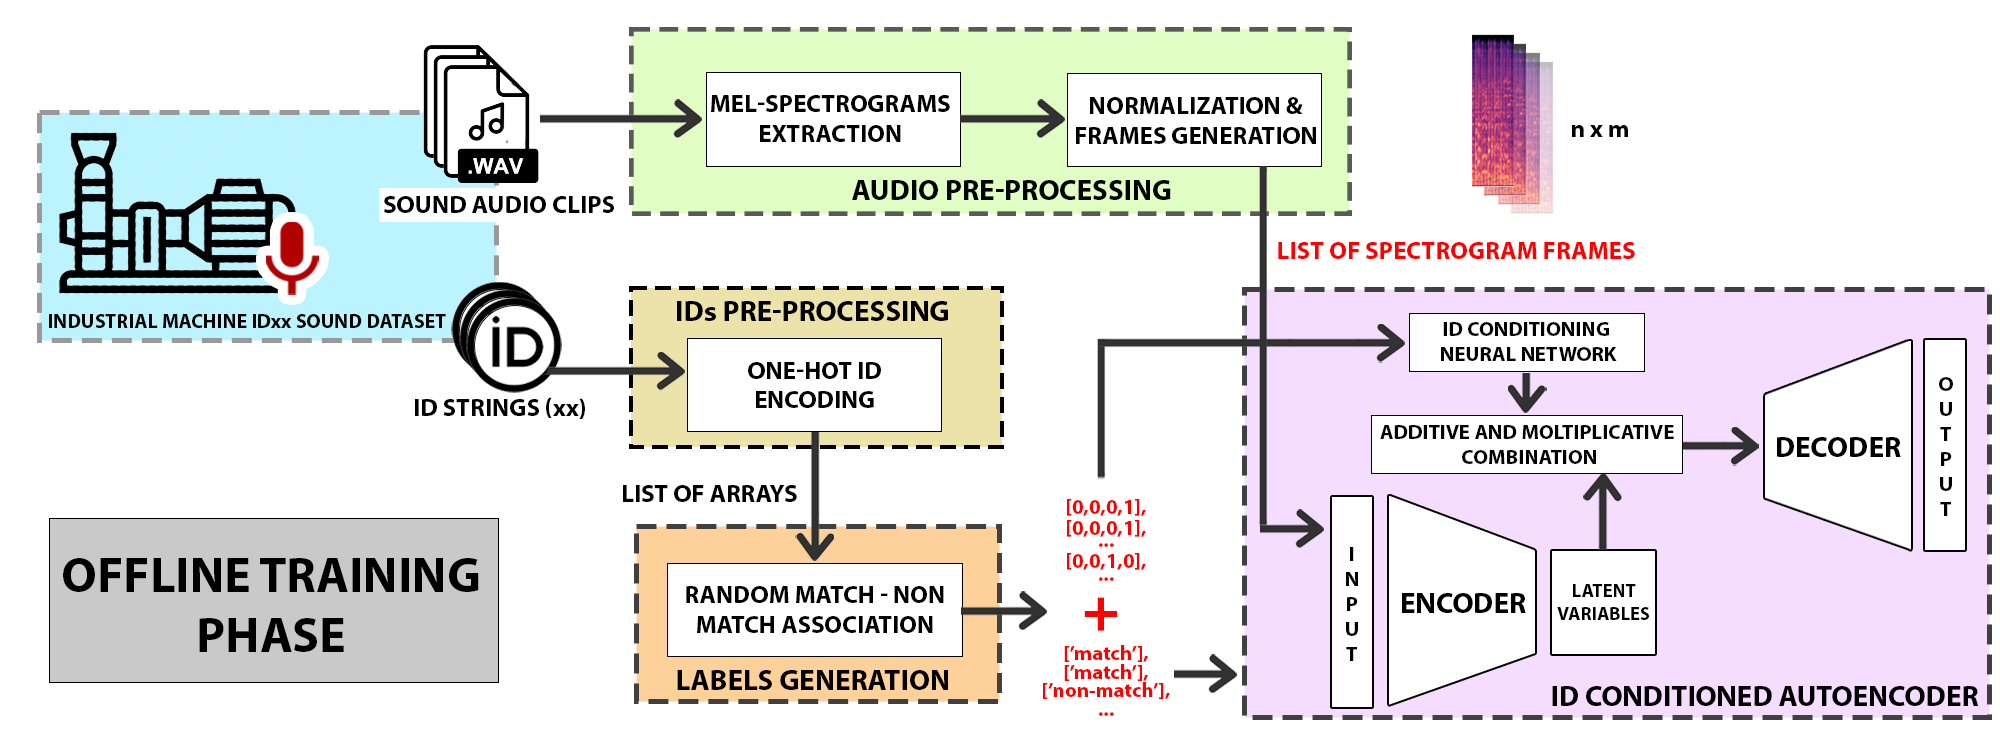
\includegraphics[scale=0.2]{TESI DI FIORE/img/offline-architecture.png}
\centering
\caption{Overview of offline training phase of the proposed ASD system.}
\label{offline-asd-system}
\end{figure}
This phase is responsible of the training of an autoencoder. The training process must be done in offline manner with the use of a pre-collected normal audio clips which belong to machines of the same type. In addition to the dataset, analyzing the Figure \ref{offline-asd-system}, other components can be noticed: the Audio Pre-Procesing block, the IDs Pre-Processing block, the Label Generation block and the ID Conditioned Autoencoder. The first three parts prepare the dataset for training process, which it is executed in the last one.
\subsubsection{Dataset Structure}
In addition to audio clips, the dataset must provide the IDs used to identify particular versions of $M$, embedding them into clips filenames (with \textit{.wav} extension) or in a separated file (obviously maintaining a one-to-one correspondence with audio files). Definitely, the data should be structured in pairs composed by audio clips plus an identifier.
\subsubsection{Offline Audio Pre-Processing}
This part of the framework is responsible of audio clips transformation, a necessary operation to make them ready for the neural network learning process, executed into the ID Conditioned Autoencoder block. There are two different components in this block:
\begin{itemize}
    \item {\textit{Mel-Spectrogram extractor} receives input audio clips and produces corresponding log-mel-scale spectrograms in output.}
    \item {\textit{Normalization and Frame generator} executes normalization on all spectrograms extracted and then it produces, from log-mel-spectrogram received in input, $n \times m$ overlapping frames with segmentation. Normalization is done between all spectrograms with the same ID. For example, in case of min-max normalization, the number of maximum and minimum values is equal to the number of different IDs. }
\end{itemize}
A little digression should be made about what these spectrograms are and how the first block calculate them. A signal is a variation in a certain quantity over time and for audio this quantity is air pressure, sampled by microphones with a particular rate (in the order of kHz). The Fast Fourier Transform (FFT) is an algorithm that allows the decomposition of a signal into its individual frequencies and frequency amplitudes, converting it from the time domain into the frequency domain (generating the spectrum). The Short-Time Fourier Transform (STFT) allows the representation of signals spectrum as they vary over time (generating the spectrogram). As audio signals frequency content varies over time (non-periodic signals), STFT is applied, because it is a FFT computed on overlapping windowed segments of the signal (Figure \ref{sftf}).\\
\begin{figure}[ht]
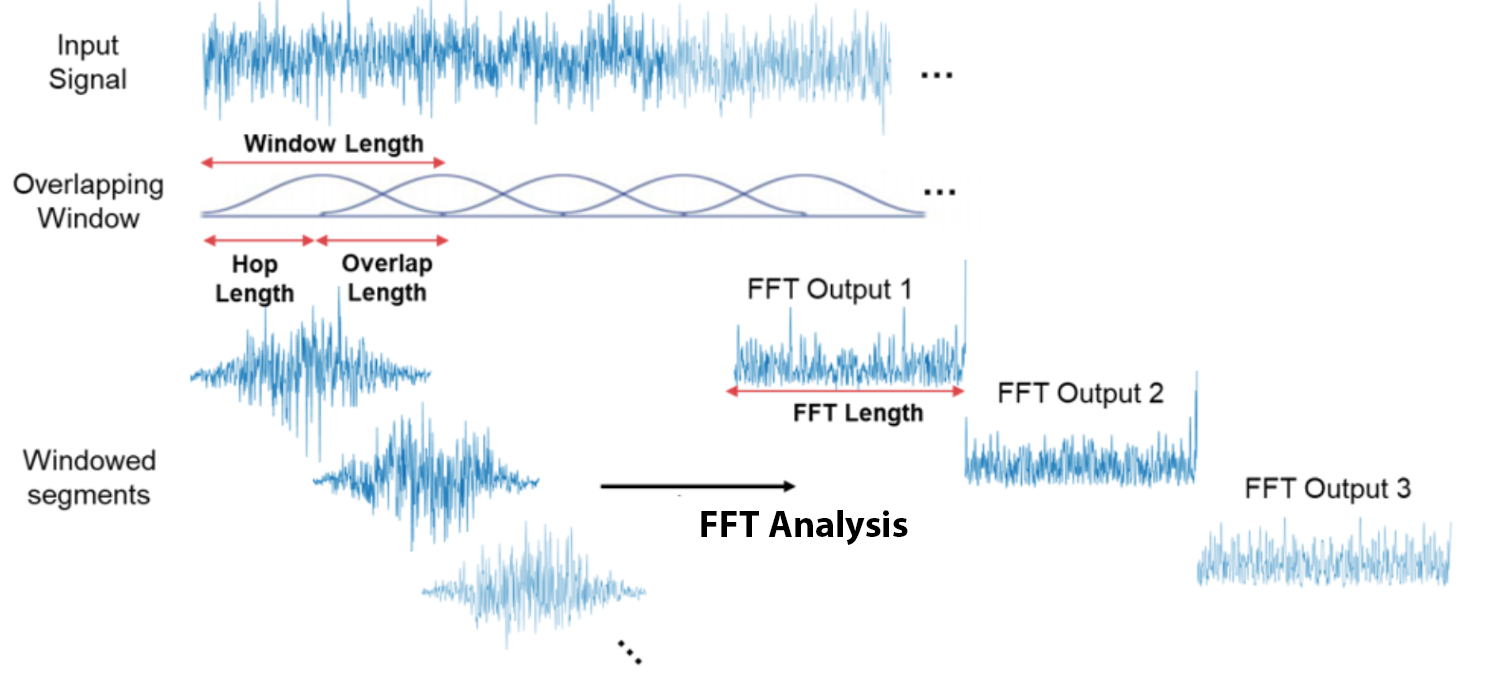
\includegraphics[scale=0.4]{TESI DI FIORE/img/STFT.png}
\centering
\caption{Overview of the STFT process.}
\label{sftf}
\end{figure}
Spectrograms usually present time on the x-axis, frequencies on the y-axis and amplitudes are indicated by colors. Log-mel-spectrograms are spectrograms in which the frequencies on y-axis are represented using the mel-scale and the amplitudes are expressed in Decibel (dB). With respect to the normal scale, the mel-scale is a scale of pitches judged by listeners to be equal in distance one from another. The most important parameters involved into this transformation process are the length of the window used for STFT ($n\_fft$), the length of the overlap between two successive windows ($hop\_length$) and the number of bins used for the transformation into the mel scale ($n$).
In the Figure \ref{features-extraction} a more detailed graphical view of what this block does is illustrated.
\begin{figure}[ht]
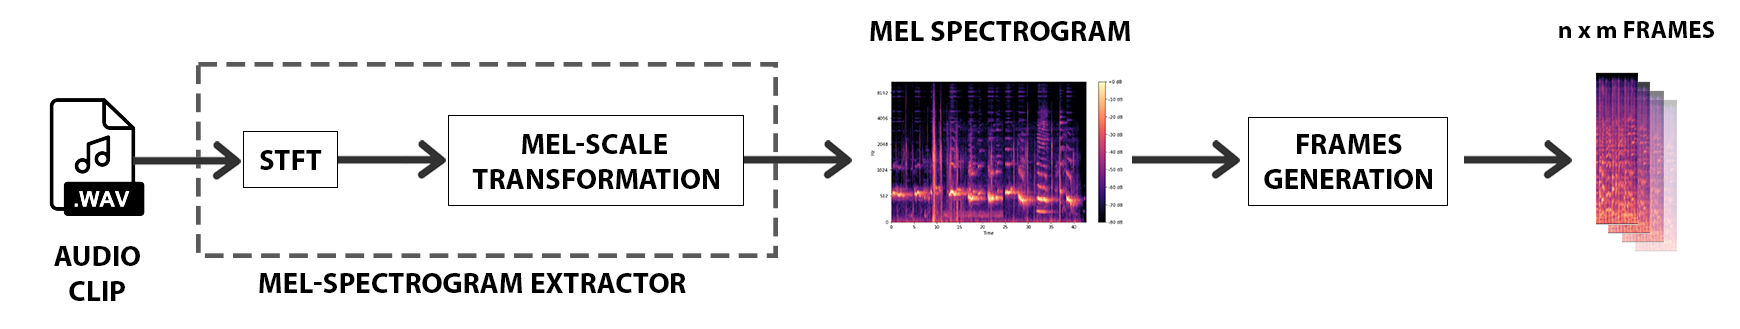
\includegraphics[scale=0.5]{TESI DI FIORE/img/FeatureExtraction.png}
\centering
\caption{Features extraction block}
\label{features-extraction}
\end{figure}
In the offline phase, $n \times m$ frames are generated from all $n \times q$ spectrograms of the training set, in order to build a new, pre-processed dataset ready for training process.
\subsubsection{IDs Pre-Processing}
This block receives in input a string, the machine ID associated to each audio clip, and converts it to a binary sequence, whose length depends by the number of different versions of $M$. This is done by the One-Hot Encoder. One-hot encoding is a technique used to convert some categorical or nominal features in order to make them compatible with training algorithm. Here ID strings are converted. Let's take an example. Supposing to have a machine $M$ and that there are four different versions of it, identified as $ID00$, $ID01$, $ID02$, $ID03$, one-hot encoder converts these strings into $[0,0,0,1]$, $[0,0,1,0]$, $[0,1,0,0]$ and $[1,0,0,0]$, respectively. The length of binary sequences is four because four is the number of versions in this case. This operation arranges the IDs to be inputs of the ID Conditioning Neural Network, better explained in the next sections. In conclusion, since each audio file spectrogram is segmented in frames, this block must ensure that those extracted from the same spectrogram are associated to the same binary sequence.
\subsubsection{ID Conditioned Autoencoder}
This part of the architecture is obviously the most important one. It receives in input three lists: the list of spectrogram frames, the list of one-hot-encoded ID arrays and the list of strings produced by Label Generator. The latter is used for the loss calculation during the training process, so that it is not a real input of the neural network (the details of what this block does are reported in the next section). In this block there are two main components: the autoencoder, composed by an encoder and a decoder, which receives the spectrogram frames in input, and the ID Conditioning Neural Network, which receives ID binary sequences. Following there is a mathematical representation of these components \cite{18IDConditionedAutoEncoder}:
\begin{itemize}
    \item {Encoder $E: \mathcal{X} \rightarrow \mathcal{Z}$ which maps the input $X$ from $\mathcal{X}$ into its encoded version $Z = E(X)$;}
    \item {Decoder $D:  \mathcal{Z} \rightarrow \mathcal{X}$ which takes the code from $\mathcal{Z}$ and outputs an reconstruction of $X$; }
    \item {Conditioning made by two functions $H_\gamma$ and $H_\beta: \mathcal{Y} \rightarrow \mathcal{Z}$, taking in input the one-hot encoded ID $l$ from $\mathcal{Y}$ in order to map it into $H_\gamma(l)$ and $H_\beta(l)$, with the same size as code from $\mathcal{Z}$.}
\end{itemize}
The encoder and the decoder can be created with different type of layers, like convolutional, LSTM or fully-connected dense layers. Between the encoder and the decoder there is a latent or encoded representation of the input $X$, or else $Z$. Differently from conventional autoencoders, in this architecture the autoencoders are conditional, because decoder input is not $Z$, but its mathematical combination with the output of conditioning functions: \[Decoder \; input: H(Z,l) = H_\gamma(l) \cdot Z + H_\beta(l).\] The conditioning functions $H_\gamma(l)$ and $ H_\beta(l)$ can be realized, for example, using dense layers and activation functions. In conclusion, the output of the entire autoencoder is $D(H(E(X),l))$. The goal of ID conditioning is to inform the model about the presence of different machines of the type $M$, for the recognition of their different normal behaviours. In general, anomalous sound of a machine $M$ with ID $x$ could be similar to normal sound of machine $M$ with ID $y$ and this could generate some false negative (FN). Moreover, normal sound of a machine $M$ with ID $w$ could be different from normal sound of a machine $M$ with ID $z$ and this could generate some false positive (FP). These two situations happen because the autoencoder is unable to separate different machine versions normal behaviour. The key concept is that the autoencoder must be trained to reconstruct normal audio spectrograms placed input only if the provided ID is correct. With this assumptions, after the training, if a normal test sample is placed in input, a low reconstruction error (in terms of mean absolute error or mean squared error) is expected, while if there is an anomalous one, an high reconstruction error is generated, even if this anomalous behavior is similar to a normal behaviour of another machine, thanks to the presence of the ID. The similarity problem is so resolved by the presence of the ID. 
\subsubsection{Label Generation}
At this point a question arises: are the only ID conditioning operations enough for this task? The answer is no because is necessary to edit the training process to help the autoencoder in the recognition of the relationship between IDs and audio clips. For this reason there is the Label Generation block. This block, for each frame, randomly changes with a probability $1-\alpha$ the correct associated ID binary sequence and it adds the string \textit{match} or \textit{not-match} on the basis of decisions. For example if there are 100 audio clips and $\alpha$ is 0.75, 75 audio clips will be associated to the correct ID sequence, the remaining 25 will be associated to a random one, from those available (so that frames belonging to the same spectrogram have the same ID binary sequence and the same string). Moreover, in order obtain what it has been just described, a new loss must be tuned and used in training steps because the classical difference between the encoder input and the decoder output is not enough. In fact, to allow a good reconstruction of the input only when the associated ID is correct, during the training, if the label is \textit{match} the loss function must be calculated in classical way as $||D(H(E(X),l)) - X||$,
while if the label is \textit{not-match} the loss function must be calculated using an arbitrary value C: $||D(H(E(X),l)) - C||$.
In conclusion, when the input spectrogram frames are associated to wrong IDs, the autoencoder will generate an high reconstruction error.
\subsection{Online Operation Phase}
\begin{figure}[ht]
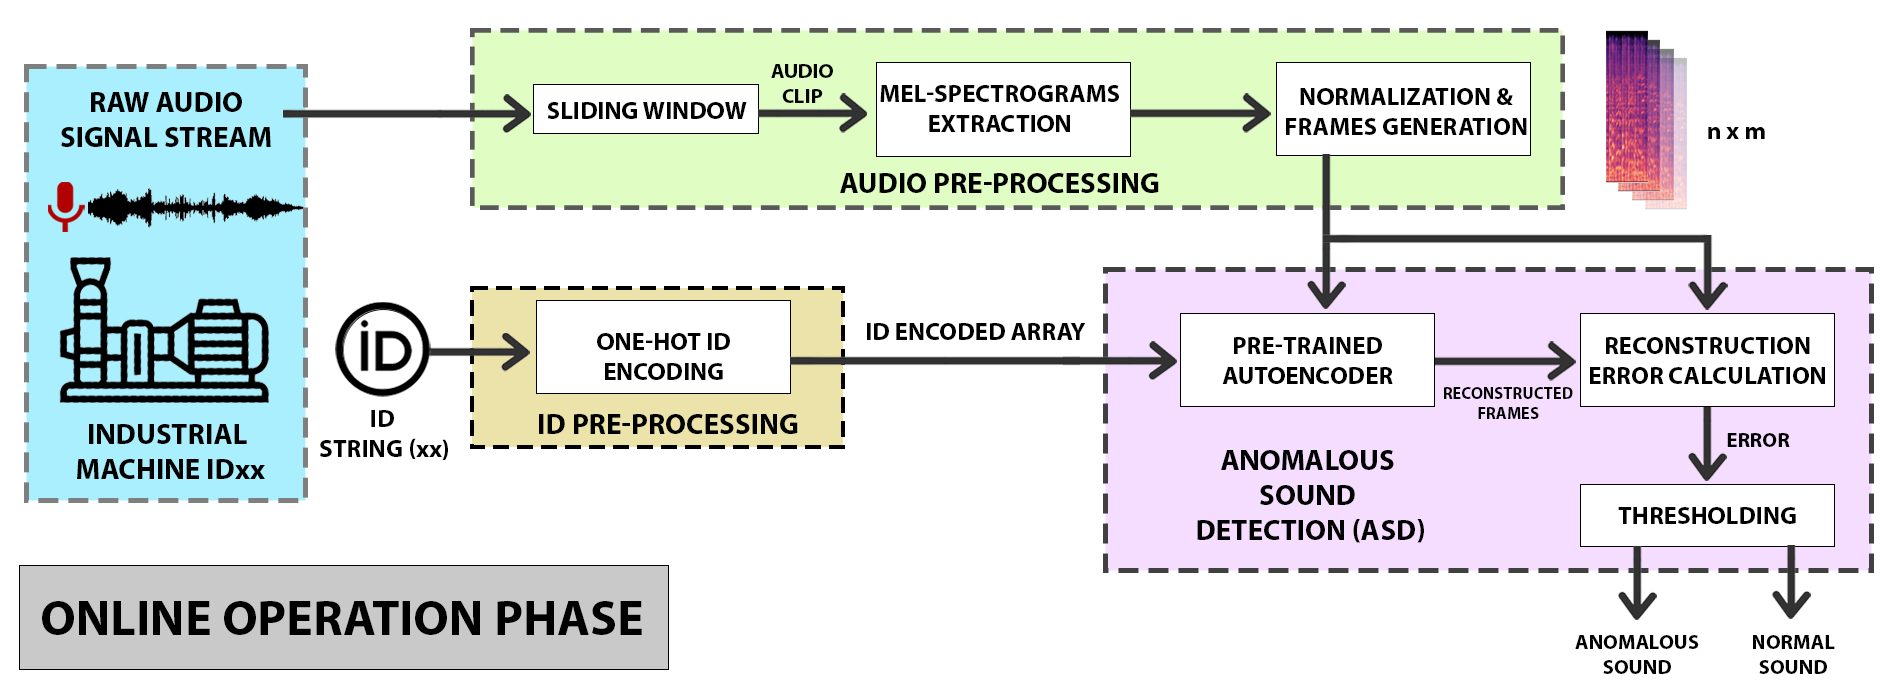
\includegraphics[scale=0.9]{TESI DI FIORE/img/online-architecture.png}
\centering
\caption{Overview of online operating phase of the proposed ASD system.}
\label{online-asd-system}
\end{figure}
The architecture used for online operation phase is very similar to the part just described, except for few components. This part of the architecture is meant for an effective and an operative use on field, since the left part of the Figure \ref{online-asd-system} shows that there is not a dataset but a real time raw audio stream from microphones disposed around the machine $M$. As other elements have been already explored in previous sections, following  there is only a description of the new ones and those that are different: Online Audio Pre-Processing block and the Anomalous Sound Detection block. 
\subsubsection{Online Audio Pre-Processing}
It is very similar to the one presented before, with exception of the sliding window component. Because of real-time anomaly detection, there is a continuous audio stream, but the autoencoder model is implemented and trained to work with $T$ seconds audio clips. For this reason, the sliding window component takes in input the stream and samples the last $T$ seconds from it, every $h$ seconds. Next, previously obtained audio clips pass into mel-spectrogram extractor block and into the frame generator, already presented. 
\subsubsection{Anomalous Sound Detection}
This is the final block of the online part of the framework and the one that is responsible of the sound labeling as normal or anomalous. In this part three components are highlighted: the pre-trained autoencoder, the reconstruction error calculator and a threshold. The pre-trained autoencoder is the result of the operations made by the offline part of the architecture. The reconstruction error calculator takes in input the output of the autoencoder and its input in order to evaluate the difference between them. This operation is made for each frame of the spectrogram associated to the audio clip (sampled from the stream) and then an average of recostruction errors is calculated for the comparison with the threshold. In fact, the threshold is used to establish if the average reconstruction error is high enough to classify clips as anomalous. The threshold could be chosen using reconstruction errors of training samples or using different approaches based on ROC curves, like the one presented at the end of Chapter 4.
\section{Hyperparameters}
In order to give a better idea related to the hyperparameters of the proposed model, following there is a summary of the most important ones:
\begin{itemize}
    \item {\textit{C}: the constant vector that must be reconstructed by the autoencoder when the provided ID is wrong;}
    \item {$\alpha$: the percentage of correct frame-ID couples in training set;}
    \item {\textit{NUM\_CONDITIONING\_LAYERS}: number of layers of the conditioning neural network;}
    \item {\textit{NUM\_CONDITIONING\_NEURONS}: number of neurons used in the the conditioning layers of the neural network and also the dimension of the encoded input generated by the encoder.}
\end{itemize}
Clearly, because of the architecture is compatible with different implementations of autoencoder layers, other hyperparameters that arise from them should be taken in consideration. Moreover, there are other hyperparameters, such as learning rate, batch size and number of epochs, which are not dependent on the proposed architecture but affect the training phase of the model.
\section{Implementation technologies}
In this section, some implementation details about the proposed model are given. The model was implemented in Python 3. Used technologies and libraries are:
\begin{itemize}
    \item {Google Colab\footnote{http://colab.research.google.com}: Colab notebooks are Jupyter notebooks that run in the cloud and are highly integrated with Google Drive, making them easy to set up, access, and share;}
    \item {Tensorflow\footnote{https://www.tensorflow.org}: it is an end-to-end open source platform for Machine Learning;}
    \item {Keras\footnote{https://keras.io}: it is an open source Deep Learning API written in Python3;}
    \item {NumPy\footnote{https://numpy.org}, used to work in an efficient way with arrays;}
    \item {SciKit-Learn\footnote{https://scikit-learn.org/stable/}, a machine learning library, containing simple and efficient tools for predictive data analysis;}
    \item {Librosa\footnote{https://librosa.org}, a Python library for audio and music processing.}
\end{itemize}



\chapter{Conclusion}
As widely seen, anomaly detection is a data-driven approach for predictive maintenance. Since it gives the possibility to avoid downtime, to reduce costs related to unnecessary operations and to optimize maintenance procedures, in last years a lot of approaches have been developed and studied by researches. In this work, after a state-of-art on autoencoders solutions for anomaly detection task, a conditional autoencoder based framework has been presented to face unsupervised anomalous sound detection. Chapter 3 and Chapter 4 show, respectively, the details of the proposed framework components and the experiments made with it, demonstrating that the involvement of machine identifiers (conditioning) into the autoencoder learning process enables models training on sounds belonging to different machines of the same type (like different pumps), improving their detection capabilities. Moreover, the experimental part of the work shows that the conditioning can be done with a classical neural network, which is also compatible with the various types of encoder-decoder layers. To demonstrate this, experiments have been conducted on DCASE 2020 Task 2 Challenge dataset, which is already arranged to face the task in unsupervised way, replicating a real scenario in which normal sound clips represent most of the available data for training phase.\\
Literature results and those collected during the experiments are really promising but improvements can still be made. In fact, regarding possible future works, in addition to a more complete hyperparameter optimization, different types of conditioning networks and operations could be attempted, together with the application of some pre-processing operations to get better training performances, like noise reduction, with the aim of reducing the audio clips background noise surely present in factory environments. Moreover, audio data augmentation techniques (like pitching, time-shifting, etc) could improve the training results. Obviously, this study could be also extended by the involvement of other, innovative, neural networks, like Variational Autoencoders (VAE) or Generative Adversarial Networks (GAN). In conclusion, as the models are trained on audio clips recorded from different machines of the same type, in order to reach better performances, ensemble approaches should be analyzed, considering that there is not an hyperparameter set that is equally good for all of them.

\bibliography{bibliography}

\bibliographystyle{plain}

\end{document}